\documentclass[aspectratio=32]{beamer}
\usepackage[utf8]{inputenc}
\usepackage[T1]{fontenc}
\usepackage{graphicx}
\graphicspath{{images/}}
\usepackage{amsmath,amssymb,amsfonts}
\usepackage[labelformat=empty]{caption}

\usepackage{listings}
\lstdefinelanguage{Lua}{
  keywords={type, true, false, function, return, nil, pcall, local, if, in, ipairs, pairs, for, while, do, else, break},
  keywordstyle=\color{blue}\bfseries,
  identifierstyle=\color{black},
  sensitive=false,
  morecomment=[l]{--},
  commentstyle=\color{purple}\ttfamily,
  stringstyle=\color{red}\ttfamily,
  morestring=[b]',
  morestring=[b]",
  sensitive=true,
  escapeinside={(*@}{@*)}
}
\lstset{ %
% columns=flexible,
% keepspaces=true,
  language=[11]C++,
  escapeinside={(*@}{@*)},
  basicstyle=\ttfamily,
  morekeywords={requires, concept}
}

\newtheorem{claim}{Proposition}

\usetheme{metropolis}
\usepackage{lmodern}

\usepackage{xeCJKfntef}
\usepackage{xeCJK}
\defaultfontfeatures{Mapping=tex-text}

\newcommand\SepLine{{\noindent\color{gray}\rule[0.25\baselineskip]{\textwidth}{1pt}} \par}

\begin{document}

\title   {OpenResty 项目模块化最佳实践}
\subtitle{更优雅的组织 OpenResty 项目模块}
\author  {张金政 \\ \texttt{tianchaijz@gmail.com}}
\date    {December 23, 2017\hfill
\includegraphics[width=0.3\textwidth]{netease}}
\maketitle

\begin{frame}[standout]
  \only<1>{                                                                   }
\end{frame}

\begin{frame}{ngx\_lua 模块配置指令执行顺序和阶段}
\begin{center}
  \begin{figure}[htlp]
    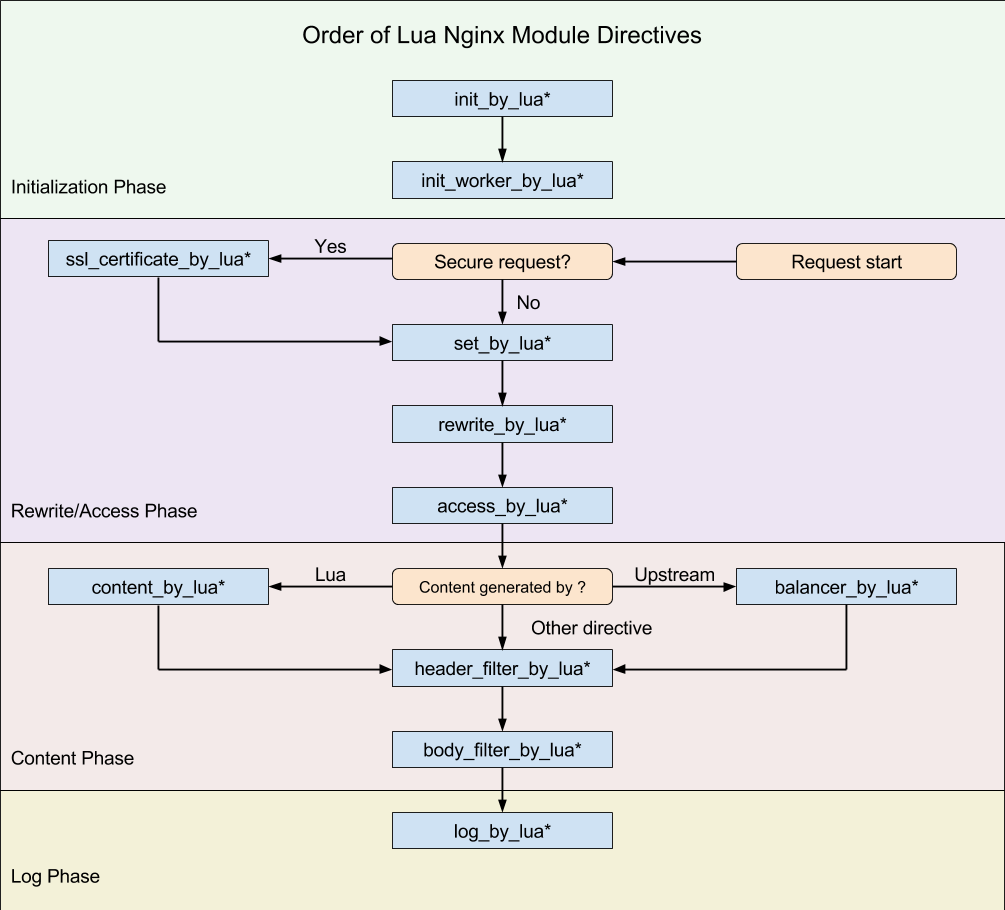
\includegraphics[width=0.7\textwidth, height=0.8\textheight]{order.png}
    \captionsetup{labelformat=empty}
    \caption{https://github.com/openresty/lua-nginx-module}
  \end{figure}
\end{center}
\end{frame}

\begin{frame}[fragile]{一个简单的鉴权网关}
\small
\begin{lstlisting}[language=lua]
-- module access
local _M = {}

function _M.check()
    -- ...
end

return _M
(*@\pause{}@*)
(*@\SepLine@*)
location / {
    access_by_lua_block {
        require("mod.access").check()
    }
}
\end{lstlisting}
\end{frame}

\begin{frame}[standout]
  \only<1>{复杂一点                                                           }
\end{frame}

\begin{frame}[fragile]{一个复杂的网关}
\small
\begin{lstlisting}[language=lua]
location / {
    rewrite_by_lua_block {
        if ngx.is_subrequest then
            return
        end
        -- ...
    }

    access_by_lua_block {
        -- module access
        -- other features
    }
}
\end{lstlisting}
\end{frame}

\begin{frame}[fragile]{一个复杂的网关}
\begin{center}
  \begin{figure}[htlp]
    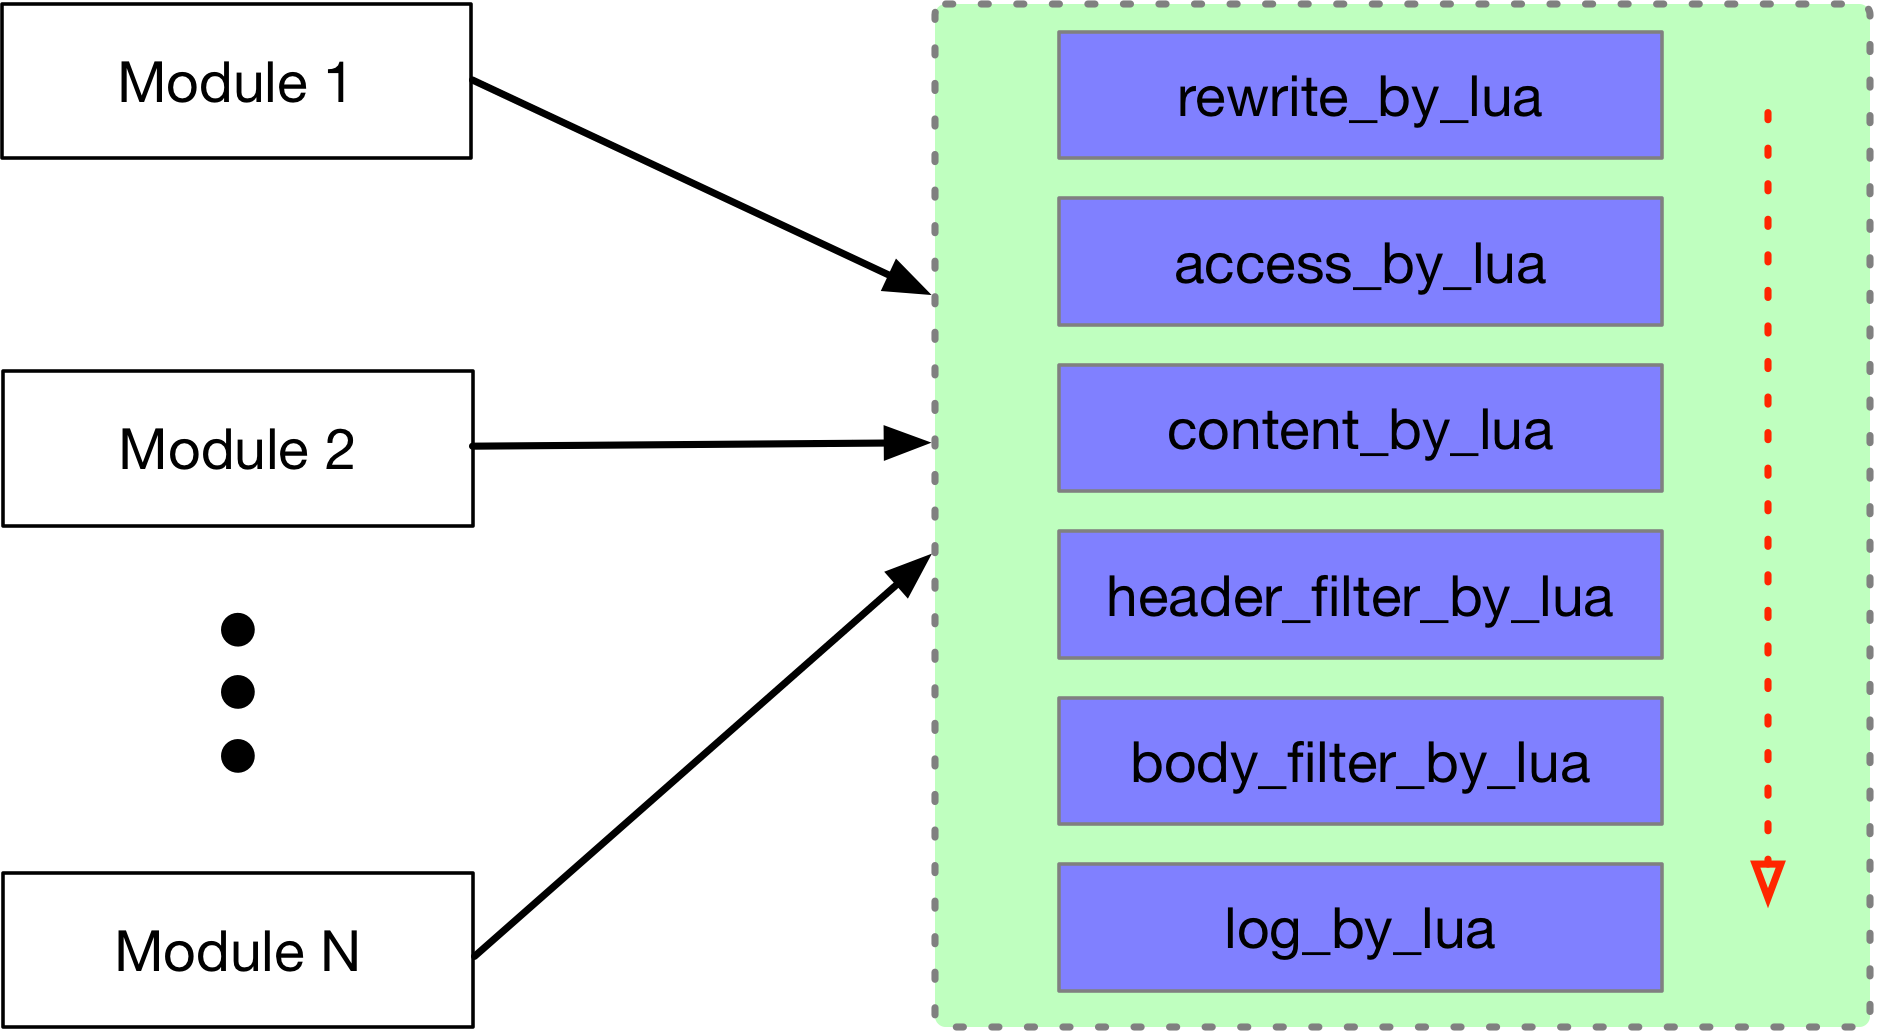
\includegraphics[width=0.9\textwidth]{complex_bad.png}
    \caption{复杂的模块调用,耦合度高,不灵活}
  \end{figure}
\end{center}
\end{frame}

\begin{frame}{缺点}
\begin{itemize}
  \item 模块之间耦合度高
  \item 模块组织不灵活
  \item 很多复杂请求不好处理,无法发挥 OpenResty 的威力
\end{itemize}
\end{frame}

\section{那么问题来了}

\begin{frame}[standout]
  \only<1>{\alert{增删}一个模块                                               }
  \only<2>{ 其他 $location$ 需要处理\alert{类似}的逻辑                        }
  \only<3>{ \Huge{\alert{$subrequest$}}                                       }
\end{frame}

\section{模块框架}

\begin{frame}[standout]
  \only<1>{ 借鉴了 NGINX 的模块机制,将\alert{模块调用关系}组织成一个链表     }
  \only<2>{ \alert{对请求分类},将请求处理流程注册到框架中                    }
  \only<3>{ 在主请求中进行\alert{路由}                                        }
\end{frame}

\begin{frame}
\begin{center}
\alert{\href{https://github.com/openresty-fan/lua-resty-master}{lua-resty-master}}\\[1.5em]
102 行 Lua 代码,简单强大
\end{center}
\end{frame}

\begin{frame}{模块方法}
\begin{itemize}
  \item new
  \item run
  \item exec
  \item set\_type
  \item next\_handler
  \item \alert{$export$}
\end{itemize}
\end{frame}

\begin{frame}[fragile]{一个简单的鉴权网关}
\small
\begin{lstlisting}[language=lua]
local MODULE = "http.mod.access"

local core = require "resty.master.core"

local function check(r)
    -- do check here
    return r:next_handler(MODULE)
end

return {
    [core.ACCESS_PHASE] = { handler = check }
}

return _M
\end{lstlisting}
\end{frame}

\begin{frame}[fragile]{一个简单的鉴权网关}
\small
\begin{lstlisting}[language=lua]
-- lua config
local _M

_M.handlers = {
    main = {
        "http.mod.access", -- access
    },
}

return _M
\end{lstlisting}
\end{frame}

\begin{frame}[fragile]{一个简单的鉴权网关}
\small
\begin{lstlisting}[language=lua]
init_worker_by_lua_block {
    local config = require "config"
    local request = require "resty.master.request"
    for typ, hs in pairs(config.handlers) do
        request.register(typ, hs)
    end
}
\end{lstlisting}
\end{frame}

\begin{frame}[fragile]{一个简单的鉴权网关}
\small
\begin{lstlisting}[language=lua]
location / {
    access_by_lua_block {
        local request = require "resty.master.request"
        local r = request.new("main")
        r:run(r.ACCESS_PHASE)
    }
}
\end{lstlisting}
\end{frame}

\begin{frame}[standout]
新增加的模块只需配置一下
\end{frame}

\begin{frame}[fragile]{一个简单的鉴权网关}
\small
\begin{lstlisting}[language=lua]
-- lua config
local _M

_M.handlers = {
    main = {
        "http.mod.access", -- access
        "http.mod.finalize", -- access (*@\only<2>{\hfill\small{\emph{只需配置}}}@*)
    },
}

return _M
\end{lstlisting}
\end{frame}

\begin{frame}[fragile]{一个复杂的网关}
\scriptsize
\begin{lstlisting}[language=lua]
-- lua config
local _M

_M.handlers = {
    main = {
        "http.mod.router", -- rewrite
        "http.mod.access", -- access
        "http.mod.finalize", -- access
    },
    ["@subrequest"] = {
        "http.mod.subrequest" -- rewrite
    },
    ["@bypass"] = {
        "http.mod.finalize", -- access
    },
    ["@internal"] = {
        -- header_filter
        { "http.mod.common", { [HEADER_FILTER] = true } },
    },
}

return _M
\end{lstlisting}
\end{frame}

\begin{frame}[fragile]{一个复杂的网关}
\scriptsize
\begin{lstlisting}[language=lua]
local MODULE = "http.mod.router"

local core = require "resty.master.core"

local function route(r)
    if ngx.is_subrequest then
        return r:exec("@subrequest")
    end

    if (*@$expr$@*) then
      return r:exec("@bypass")
    end

    return r:next_handler(MODULE)
end

return {
    [core.REWRITE_PHASE] = { handler = route }
}
\end{lstlisting}
\end{frame}

\begin{frame}[fragile]{一个复杂的网关}
\scriptsize
\begin{lstlisting}[language=lua]
rewrite_by_lua_block {
    local r = require("resty.master.request").new("main")
    ngx.ctx.request = r
    r:run(r.REWRITE_PHASE)
}

access_by_lua_block {
    local r = ngx.ctx.request
    r:run(r.ACCESS_PHASE)
}
\end{lstlisting}
\end{frame}

\begin{frame}[fragile]{一个复杂的网关}
\begin{center}
  \begin{figure}[htlp]
    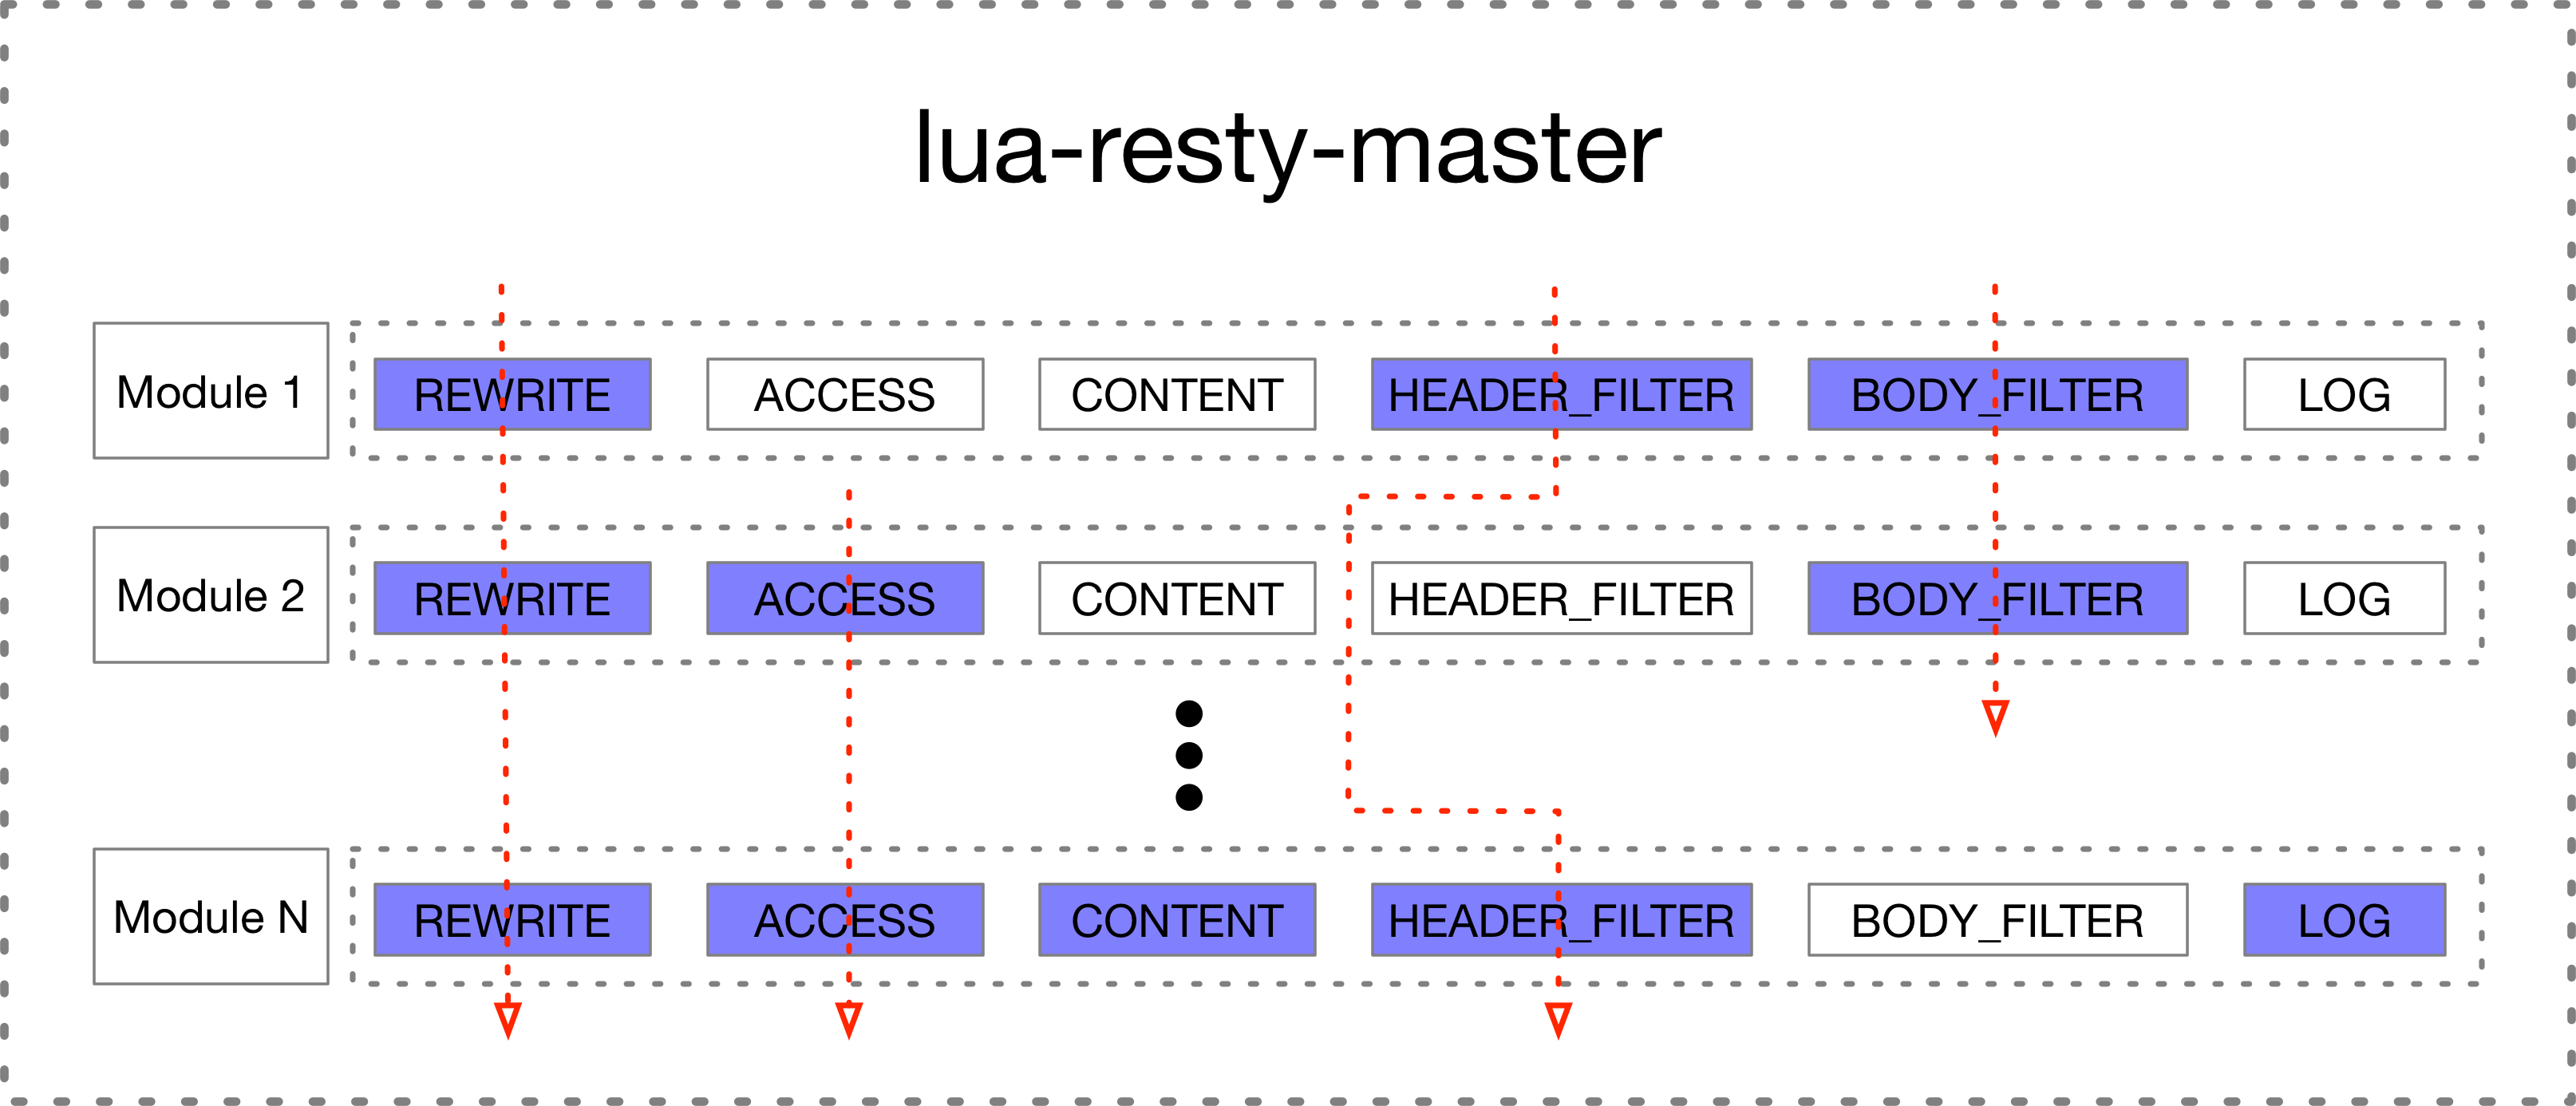
\includegraphics[width=0.9\textwidth]{complex_good.png}
    \caption{复杂的模块调用,耦合度低,灵活}
  \end{figure}
\end{center}
\end{frame}

\begin{frame}{优点}
\begin{itemize}
  \item \lstinline|ngx_lua hooks| 都变成了占位符,无任何逻辑
  \item 配合 \lstinline|ngx.exec| 能发挥出 OpenResty 更大的威力
  \item 项目组织完全配置化
\end{itemize}
\end{frame}

\section{为所欲为}

\begin{frame}{只需修改配置}
\begin{itemize}
  \item \alert{增删}一个模块
  \item 其他 $location$ 需要处理\alert{类似}的逻辑
  \item $subrequest$
\end{itemize}
\pause{}
\centerline{\LARGE 这些问题已不存在}
\end{frame}

\begin{frame}[standout]
面向配置编程
\end{frame}

\section{优点不止这些}

\begin{frame}[standout]
  \only<1>{ 让开发者重新审视自己的模块 }
  \only<2>{ 让开发精力集中到项目架构中 }
  \only<3>{ 快乐编程 }
\end{frame}

\section{小技巧}

\begin{frame}{小技巧}
\begin{itemize}
  \item 把处理好的 NGINX 变量都放在 $request$ 对象中
  \item 一个专门的 $finalize$ 模块做请求处理收尾,设置 NGINX 变量
  \item \lstinline|ngx.exec| 时使用 $freelist$ 算法优雅的保存 \lstinline|ngx.ctx| 变量
\end{itemize}
\end{frame}

\begin{frame}[fragile]{优雅的保存 \lstinline|ngx.ctx|}
\small
\begin{lstlisting}[language=lua]
local stash_ctx = require("mod.ngx_ctx").stash
local function go(r)
    stash_ctx() -- save ngx.ctx
    -- r:set_type("fetch")
    return ngx.exec("/content")
end
(*@\pause{}@*)
(*@\SepLine@*)
location /content {
    content_by_lua_block {
        require("mod.ngx_ctx").apply()
        local r = ngx.ctx.request
        r:run(r.CONTENT_PHASE)
    }
}
\end{lstlisting}
\end{frame}

\begin{frame}[fragile]{序列化 \lstinline|request| 对象}
\small
\begin{lstlisting}[language=lua]
local function serialize(r)
    local rdata = {}
    for k, v in pairs(r) do
        if is_str(k) and string_sub(k, 1, 1) ~= "_"
            and not is_func(v) then
            rdata[k] = v
        end
    end

    return cmsgpack.pack(rdata)
end
\end{lstlisting}
\end{frame}

\section{使用案例}

\begin{frame}[fragile]{文件分片}
\begin{itemize}
  \item 优雅的隔离 $subrequest$
\end{itemize}
\end{frame}

\begin{frame}[fragile]{视频 seek}
\begin{itemize}
  \item 获取视频元数据 + 视频 $seek$ 后的内容
\end{itemize}
\end{frame}

\begin{frame}[fragile]{视频 seek}
\begin{center}
  \begin{figure}[htlp]
    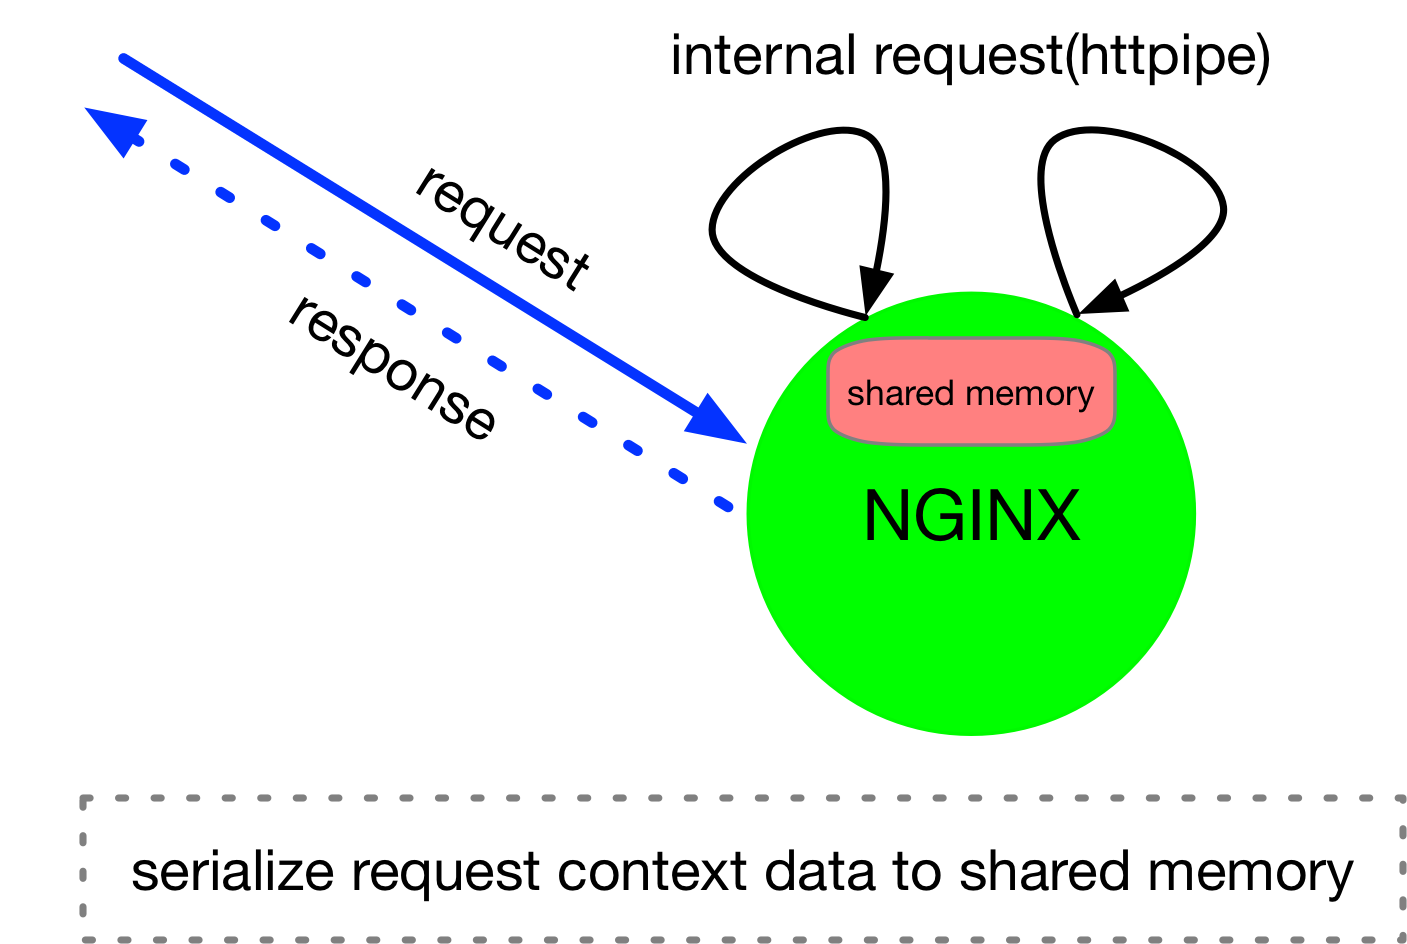
\includegraphics[width=0.9\textwidth]{seek.png}
  \end{figure}
\end{center}
\end{frame}

\begin{frame}[fragile]{CDN 私有请求}
将私有请求直接路由到一个没有权限校验的处理流程中
\begin{itemize}
  \item 绕过鉴权
  \item 文件预热
  \item 刷新 URL 转换
\end{itemize}
\end{frame}

\section{推而广之}

\begin{frame}[standout]
在其他非 OpenResty 项目中尝试使用这种模块机制
\end{frame}

\begin{frame}
\begin{center}
https://github.com/openresty-fan/lua-resty-master \\[2em]
Questions?
\end{center}
\end{frame}

\begin{frame}[standout]
广告
\end{frame}

\end{document}
